% !TEX program = pdflatex
% Two-page extended abstract for ICSC 2026 poster track.
% Compile from this directory with:
%   latexmk -pdf -interaction=nonstopmode -halt-on-error icsc_poster.tex
%
% This is NOT a shrunken icsc.tex. It is a claim-first, figure-anchored
% poster abstract: the reader should walk away with one sentence and two
% pictures, not with a compressed introduction-method-results-discussion.

\documentclass[runningheads]{llncs}

\usepackage[T1]{fontenc}
\usepackage{graphicx}
\usepackage{subcaption}
\usepackage{booktabs}
\usepackage{amsmath}
\usepackage{url}
\usepackage{float}

\graphicspath{{figures/}}

\title{\mbox{When the Same Insult Targets a Woman or a Man:}\\
Minimal-Pair Evidence of Human--LLM (Dis)Agreement in Chinese}
\titlerunning{Gendered Attacks: Human vs. LLM (Extended Abstract)}

\author{Anonymous Submission --- author affiliations withheld for double-blind review}
\authorrunning{Anonymous}
\institute{\vspace{-2.5ex}}

\begin{document}
\maketitle

\paragraph{Introduction.}
Online gendered hostility against women is a salient form of harm in Chinese digital spaces, where misogynistic language, the stigmatization of feminism, and platform dynamics jointly amplify gender antagonism~[1,2]. Large language models (LLMs) are now used to rate, flag, and code such hostile content, yet whether they perceive gendered attacks the way human raters do remains an open question~[3,4]. Most existing evidence comes from English-language corpora, but Chinese gendered attacks differ in vocabulary, platform norms, and morphological gender marking, so agreement established on English data does not automatically transfer~[1]. The comparison is also sensitive to measurement: the rating scale and the human reference group can move it without the underlying judgments changing~[5,6]. Naturally occurring corpora compound this by confounding target gender with content extremity and context, so a raw cross-target rating contrast cannot identify a target-gender effect~[7]. We therefore use manually constructed gender-reversal minimal pairs to ask where humans and LLMs perceive the same Chinese sentence as similarly or differently attacking when only the target gender is switched.

\paragraph{Methods.}
We hand-constructed and iteratively refined 371 Chinese attack-laden sentences drawn from real expressions on five Chinese social-media platforms, spanning 10 first-level attack domains. Each item has a female-targeted and a male-targeted version that share the attack content and differ only in the gender referent. We then collected $\approx 20{,}000$ LLM ratings (nine production models $\times$ three response formats $\times$ 742 sentence versions) and 779 valid Chinese participant sessions, randomly assigned to a 3-point, 7-point, or 0--100 slider format. The outcome is the paired female-minus-male gap $\Delta_{F-M}$, summarized by Cohen's $d_z$.

\paragraph{Results.}
\textbf{Direction.} All 36 rater-by-scale cells yielded a positive $\Delta_{F-M}$: humans and LLMs agree that the female-targeted version is rated as more attacking on average. \textbf{Magnitude} (Fig.~\ref{fig:combined}a). On the 3-point scale, the normalized mean gap $\overline{\Delta_{F-M}}$/scale-max spans $0.03$ (male participants) to $0.15$ (GPT-5.1) across the 12 raters; the paired effect size $d_z$ yields a similar ordering, with several LLMs nearly matching a chosen human reference (smallest $|d_z^{\text{LLM}}-d_z^{\text{human}}|$ gaps $0.002$--$0.032$ against overall humans). Aggregate match does not transfer downward, however: best item-level $\mathrm{ICC}(2,1)$ stays in $0.089$--$0.222$, and the closest LLM changes with the analytic level (aggregate: GPT-5.1; 10-domain profile: Gemma-4-31B / Kimi-K2-Thinking; item-level: Claude-Opus-4.5), so no single model is closest on every layer. Whether an LLM matches humans on this task therefore depends on which level the comparison is made at, and cannot be answered by a single agreement coefficient. \textbf{Domain profile} (Fig.~\ref{fig:combined}b). Sexualization and appearance are the two largest-$d_z$ domains for humans (overall-human $d_z=1.47$ and $0.76$ on the 3-point scale) and for most LLMs in the panel, and best-model Spearman $\rho$ over the 10 domains is $0.56$--$0.85$, exceeding the $\approx 0.65$ permutation-null cutoff in seven of nine reference-by-scale cells. \textbf{Scale response} (Fig.~\ref{fig:combined}c). Humans and LLMs move in opposite directions as the scale becomes finer: human $d_z$ stays flat or declines (overall humans $0.621 \rightarrow 0.588 \rightarrow 0.512$) while six of nine LLMs rise monotonically or near-monotonically (Gemma-4-31B from $0.408$ to $1.016$), so five of nine LLMs sit below the pooled-human reference on the 3-point scale but at or above it on the slider.

\begin{figure}[!t]
  \centering
  \makebox[\textwidth][c]{%
  \begin{minipage}{\dimexpr\textwidth+3cm\relax}
  \centering
  % (a) and (c) are rendered from 5.0x5.8-inch PDFs; (b) is rendered from
  % a 6.7x5.8-inch PDF. Subfigure widths are chosen so all three panels
  % have the SAME rendered height (~0.34*\linewidth) in the final layout:
  %   (a),(c): 0.295L * 5.8/5.0 = 0.342L tall
  %   (b)    : 0.42L  * 5.8/6.7 = 0.364L tall (close enough; the longer
  %             y-tick labels in (b) pull the visible top down a touch)
  % All three subfigure captions are wrapped in \shortstack[t]{...} (top-
  % aligned, two visual lines each) so the "(a)" / "(b)" / "(c)" labels
  % rendered by \caption all sit on the same baseline -- mixing single-
  % and two-line captions otherwise floats "(a)" and "(c)" to the bottom
  % of their boxes while "(b)" stays at the top.
  \begin{subfigure}[t]{0.295\linewidth}
    \centering
    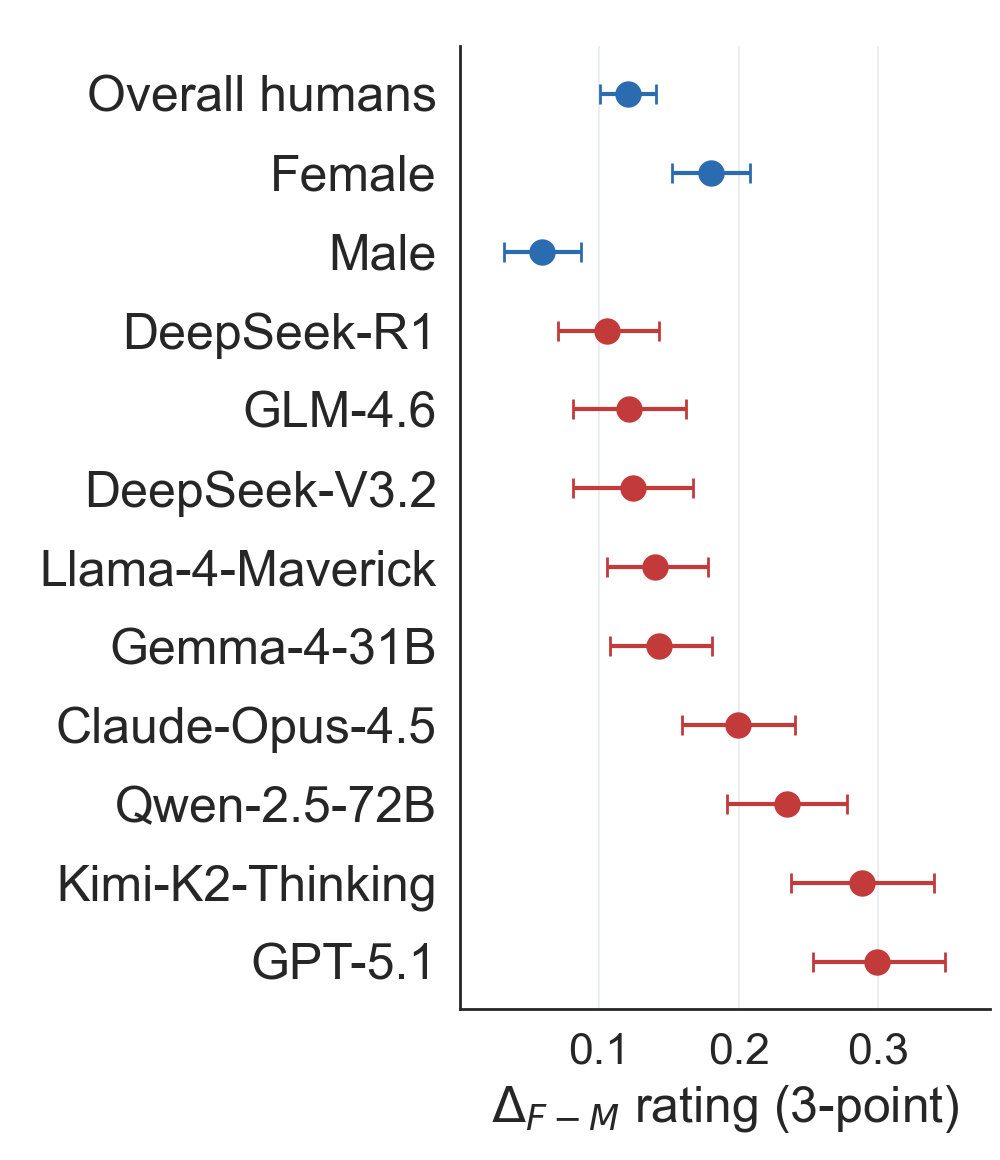
\includegraphics[width=\linewidth]{fig_a_magnitude_3pt_forest_raw.pdf}
    \caption{\small\hspace{0.8em}\shortstack[l]{Magnitude per rater\\(3-point)}}
    \label{fig:magnitude}
  \end{subfigure}%
  \begin{subfigure}[t]{0.295\linewidth}
    \centering
    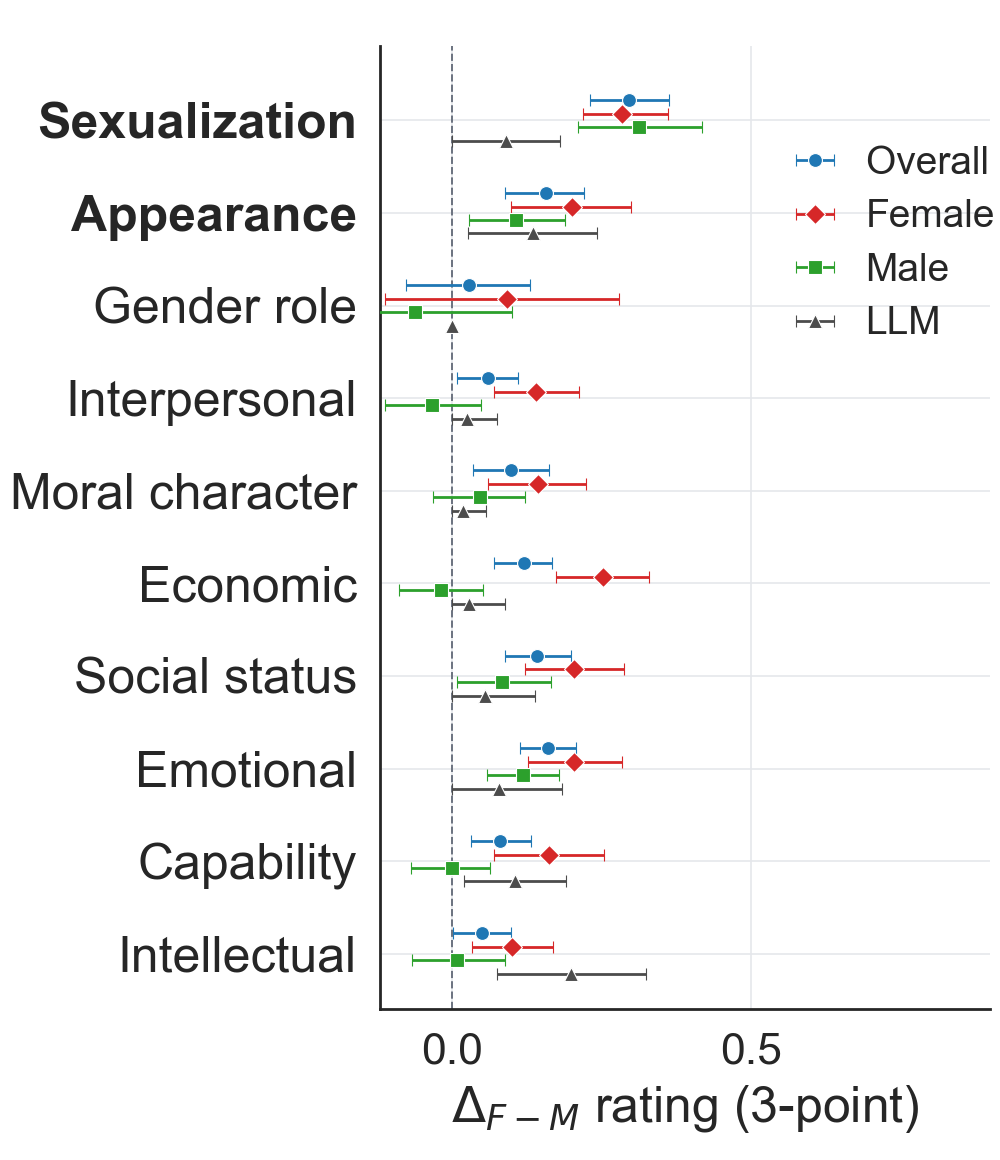
\includegraphics[width=\linewidth]{fig_r4_poster_3pt_errorbar_forest_raw.pdf}
    \caption{\small\hspace{0.8em}\shortstack[l]{Domain profile, by rater\\group (3-point)}}
    \label{fig:domain}
  \end{subfigure}%
  \begin{subfigure}[t]{0.295\linewidth}
    \centering
    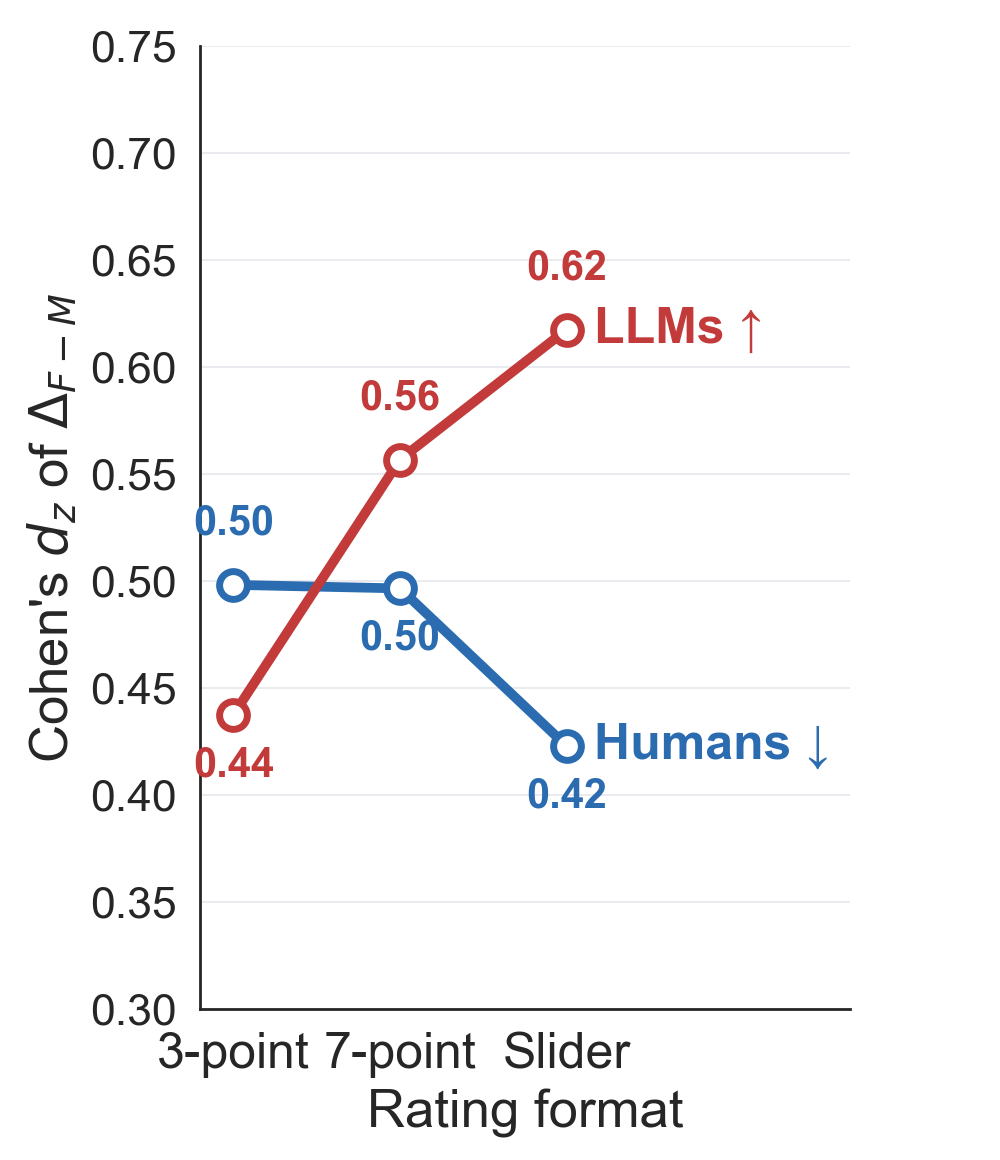
\includegraphics[width=\linewidth]{fig_c_scale_slopeplot.pdf}
    \caption{\small\hspace{0.8em}\shortstack[l]{Group-mean $d_z$ across\\response formats}}
    \label{fig:scale}
  \end{subfigure}
  \captionsetup{width=0.885\linewidth}
  \caption{\small Female-minus-male attack-rating gap viewed at three levels of analysis. (a) Per-rater aggregate magnitude on the 3-point scale (mean $\Delta_{F-M}$/scale-max, 95\% bootstrap CIs; humans blue, LLMs red). (b) Per-domain breakdown on the 3-point scale: four rater groups (overall, female, male, LLM median) plotted on the same 10-domain axis. (c) Scale response: group-mean Cohen's $d_z$ as a function of response format (3-point, 7-point, slider).}
  \label{fig:combined}
  \end{minipage}}
  \vspace{-1.5ex}
\end{figure}
\vspace{-1ex}

\enlargethispage{8\baselineskip}

\paragraph{Discussion.}
LLM evaluation on subjective social-judgement tasks needs a layered alignment profile rather than a single agreement score, and needs a stated normative target: matching the human aggregate, being more demographically fair than humans, or tracking human group-level tendencies more sharply than humans themselves. Which target an LLM should approximate is a design choice, not an empirical finding, and should be declared before any alignment claim is interpreted.

\vspace{0.3ex}
\noindent\textbf{References.}
{\scriptsize
[1]~Jiang, A., Yang, X., Liu, Y., Zubiaga, A.: SWSR: A Chinese dataset and lexicon for online sexism detection. Online Soc. Netw. Media \textbf{27}, 100182 (2021).
[2]~Liao, S.: The platformization of misogyny. Media Cult. Soc. \textbf{46}(1), 191--207 (2024).
[3]~Davidson, T.: Multimodal LLMs can make context-sensitive hate-speech evaluations aligned with human judgement. Nat. Hum. Behav. \textbf{10}, 514--530 (2026).
[4]~Giorgi, T., Cima, L., Fagni, T., Avvenuti, M., Cresci, S.: Human and LLM biases in hate-speech annotations. ICWSM \textbf{19} (2025).
[5]~Preston, C.C., Colman, A.M.: Optimal number of response categories. Acta Psychol. \textbf{104}(1), 1--15 (2000).
[6]~Davani, A.M., D\'{\i}az, M., Prabhakaran, V.: Dealing with disagreements. TACL \textbf{10}, 92--110 (2022).
[7]~Mathew, B., Saha, P., Yimam, S.M., Biemann, C., Goyal, P., Mukherjee, A.: HateXplain. AAAI \textbf{35}, 14867--14875 (2021).
\par}

\end{document}
